\documentclass{standalone}
\usepackage{tikz}
\usetikzlibrary{patterns, positioning}

\begin{document}
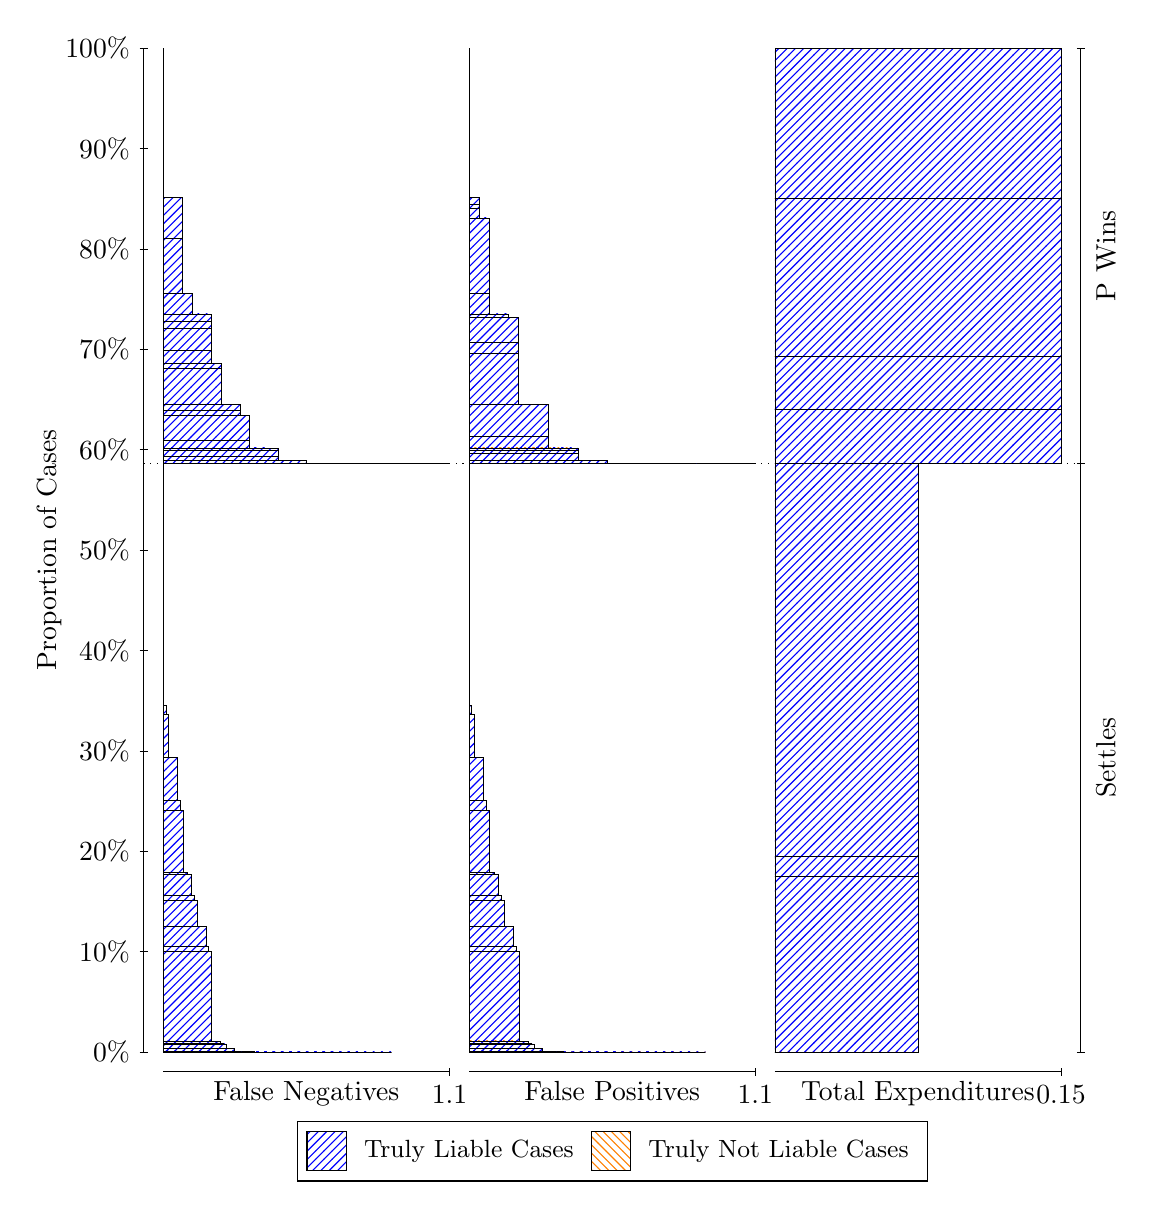
\begin{tikzpicture}
\draw[black, very thin] (1.5,1.75) -- (1.5,14.5);
\node[rotate=90, anchor=center] at (0.3, 8.125) {Proportion of Cases};
\draw[black, very thin] (1.45,1.75) -- (1.55,1.75);
\node[anchor=east] at (1.45, 1.75) {0\%};
\draw[black, very thin] (1.45,3.025) -- (1.55,3.025);
\node[anchor=east] at (1.45, 3.025) {10\%};
\draw[black, very thin] (1.45,4.3) -- (1.55,4.3);
\node[anchor=east] at (1.45, 4.3) {20\%};
\draw[black, very thin] (1.45,5.575) -- (1.55,5.575);
\node[anchor=east] at (1.45, 5.575) {30\%};
\draw[black, very thin] (1.45,6.85) -- (1.55,6.85);
\node[anchor=east] at (1.45, 6.85) {40\%};
\draw[black, very thin] (1.45,8.125) -- (1.55,8.125);
\node[anchor=east] at (1.45, 8.125) {50\%};
\draw[black, very thin] (1.45,9.4) -- (1.55,9.4);
\node[anchor=east] at (1.45, 9.4) {60\%};
\draw[black, very thin] (1.45,10.675) -- (1.55,10.675);
\node[anchor=east] at (1.45, 10.675) {70\%};
\draw[black, very thin] (1.45,11.95) -- (1.55,11.95);
\node[anchor=east] at (1.45, 11.95) {80\%};
\draw[black, very thin] (1.45,13.225) -- (1.55,13.225);
\node[anchor=east] at (1.45, 13.225) {90\%};
\draw[black, very thin] (1.45,14.5) -- (1.55,14.5);
\node[anchor=east] at (1.45, 14.5) {100\%};

\draw[black, very thin] (13.4,1.75) -- (13.4,14.5);
\draw[black, very thin] (13.35,1.75) -- (13.45,1.75);
\node[anchor=west] at (13.35, 1.75) {};
\draw[black, very thin] (13.35,9.224) -- (13.45,9.224);
\node[anchor=west] at (13.35, 9.224) {};
\draw[black, very thin] (13.35,14.5) -- (13.45,14.5);
\node[anchor=west] at (13.35, 14.5) {};

\draw[black, very thin, pattern color=blue, pattern=north east lines] (1.75,1.75) rectangle (4.6485,1.75);
\draw[black, very thin, pattern color=blue, pattern=north east lines] (1.75,1.75) rectangle (4.3219,1.75);
\draw[black, very thin, pattern color=blue, pattern=north east lines] (1.75,1.75) rectangle (4.2856,1.75);
\draw[black, very thin, pattern color=blue, pattern=north east lines] (1.75,1.75) rectangle (3.9953,1.75);
\draw[black, very thin, pattern color=blue, pattern=north east lines] (1.75,1.75) rectangle (3.959,1.75);
\draw[black, very thin, pattern color=blue, pattern=north east lines] (1.75,1.75) rectangle (3.9227,1.75);
\draw[black, very thin, pattern color=blue, pattern=north east lines] (1.75,1.75) rectangle (3.832,1.75);
\draw[black, very thin, pattern color=blue, pattern=north east lines] (1.75,1.75) rectangle (3.6324,1.75);
\draw[black, very thin, pattern color=blue, pattern=north east lines] (1.75,1.75) rectangle (3.5962,1.75);
\draw[black, very thin, pattern color=blue, pattern=north east lines] (1.75,1.75) rectangle (3.5599,1.75);
\draw[black, very thin, pattern color=blue, pattern=north east lines] (1.75,1.75) rectangle (3.5054,1.75);
\draw[black, very thin, pattern color=blue, pattern=north east lines] (1.75,1.75) rectangle (3.4691,1.75);
\draw[black, very thin, pattern color=blue, pattern=north east lines] (1.75,1.75) rectangle (3.2696,1.75);
\draw[black, very thin, pattern color=blue, pattern=north east lines] (1.75,1.75) rectangle (3.2333,1.75);
\draw[black, very thin, pattern color=blue, pattern=north east lines] (1.75,1.75) rectangle (3.197,1.75);
\draw[black, very thin, pattern color=blue, pattern=north east lines] (1.75,1.75) rectangle (3.1788,1.75);
\draw[black, very thin, pattern color=blue, pattern=north east lines] (1.75,1.75) rectangle (3.1426,1.75);
\draw[black, very thin, pattern color=blue, pattern=north east lines] (1.75,1.75) rectangle (3.1063,1.75);
\draw[black, very thin, pattern color=blue, pattern=north east lines] (1.75,1.75) rectangle (3.0155,1.7511);
\draw[black, very thin, pattern color=blue, pattern=north east lines] (1.75,1.7511) rectangle (2.9067,1.7536);
\draw[black, very thin, pattern color=blue, pattern=north east lines] (1.75,1.7536) rectangle (2.8704,1.7538);
\draw[black, very thin, pattern color=blue, pattern=north east lines] (1.75,1.7538) rectangle (2.8341,1.7543);
\draw[black, very thin, pattern color=blue, pattern=north east lines] (1.75,1.7543) rectangle (2.816,1.7543);
\draw[black, very thin, pattern color=blue, pattern=north east lines] (1.75,1.7543) rectangle (2.7797,1.7545);
\draw[black, very thin, pattern color=blue, pattern=north east lines] (1.75,1.7545) rectangle (2.7434,1.7545);
\draw[black, very thin, pattern color=blue, pattern=north east lines] (1.75,1.7545) rectangle (2.689,1.7648);
\draw[black, very thin, pattern color=blue, pattern=north east lines] (1.75,1.7648) rectangle (2.6527,1.7944);
\draw[black, very thin, pattern color=blue, pattern=north east lines] (1.75,1.7944) rectangle (2.5438,1.8526);
\draw[black, very thin, pattern color=blue, pattern=north east lines] (1.75,1.8526) rectangle (2.5075,1.8594);
\draw[black, very thin, pattern color=blue, pattern=north east lines] (1.75,1.8594) rectangle (2.4712,1.8856);
\draw[black, very thin, pattern color=blue, pattern=north east lines] (1.75,1.8856) rectangle (2.4531,1.8857);
\draw[black, very thin, pattern color=blue, pattern=north east lines] (1.75,1.8857) rectangle (2.4168,1.8907);
\draw[black, very thin, pattern color=blue, pattern=north east lines] (1.75,1.8907) rectangle (2.3805,1.8907);
\draw[black, very thin, pattern color=blue, pattern=north east lines] (1.75,1.8907) rectangle (2.3624,3.0322);
\draw[black, very thin, pattern color=blue, pattern=north east lines] (1.75,3.0322) rectangle (2.3261,3.0933);
\draw[black, very thin, pattern color=blue, pattern=north east lines] (1.75,3.0933) rectangle (2.2898,3.342);
\draw[black, very thin, pattern color=blue, pattern=north east lines] (1.75,3.342) rectangle (2.1809,3.6759);
\draw[black, very thin, pattern color=blue, pattern=north east lines] (1.75,3.6759) rectangle (2.1446,3.7341);
\draw[black, very thin, pattern color=blue, pattern=north east lines] (1.75,3.7341) rectangle (2.1083,4.0016);
\draw[black, very thin, pattern color=blue, pattern=north east lines] (1.75,4.0016) rectangle (2.0902,4.0021);
\draw[black, very thin, pattern color=blue, pattern=north east lines] (1.75,4.0021) rectangle (2.0539,4.0278);
\draw[black, very thin, pattern color=blue, pattern=north east lines] (1.75,4.0278) rectangle (2.0176,4.0283);
\draw[black, very thin, pattern color=blue, pattern=north east lines] (1.75,4.0283) rectangle (1.9995,4.8207);
\draw[black, very thin, pattern color=blue, pattern=north east lines] (1.75,4.8207) rectangle (1.9632,4.941);
\draw[black, very thin, pattern color=blue, pattern=north east lines] (1.75,4.941) rectangle (1.9269,5.487);
\draw[black, very thin, pattern color=blue, pattern=north east lines] (1.75,5.487) rectangle (1.818,6.033);
\draw[black, very thin, pattern color=blue, pattern=north east lines] (1.75,6.033) rectangle (1.7818,6.1534);
\draw[black, very thin, pattern color=orange, pattern=north west lines] (1.75,6.1534) rectangle (1.75,6.1534);
\draw[black, very thin, pattern color=blue, pattern=north east lines] (1.75,6.1534) rectangle (1.75,9.224);
\draw[black, very thin, pattern color=blue, pattern=north east lines] (1.75,9.224) rectangle (5.3833,9.224);
\draw[black, very thin, pattern color=blue, pattern=north east lines] (1.75,9.224) rectangle (5.0205,9.224);
\draw[black, very thin, pattern color=blue, pattern=north east lines] (1.75,9.224) rectangle (4.6576,9.224);
\draw[black, very thin, pattern color=blue, pattern=north east lines] (1.75,9.224) rectangle (4.5351,9.224);
\draw[black, very thin, pattern color=blue, pattern=north east lines] (1.75,9.224) rectangle (4.2947,9.2241);
\draw[black, very thin, pattern color=blue, pattern=north east lines] (1.75,9.2241) rectangle (4.2947,9.2242);
\draw[black, very thin, pattern color=blue, pattern=north east lines] (1.75,9.2242) rectangle (4.1722,9.2242);
\draw[black, very thin, pattern color=blue, pattern=north east lines] (1.75,9.2242) rectangle (3.9318,9.2263);
\draw[black, very thin, pattern color=blue, pattern=north east lines] (1.75,9.2263) rectangle (3.9318,9.2277);
\draw[black, very thin, pattern color=blue, pattern=north east lines] (1.75,9.2277) rectangle (3.8093,9.2277);
\draw[black, very thin, pattern color=blue, pattern=north east lines] (1.75,9.2277) rectangle (3.5689,9.2587);
\draw[black, very thin, pattern color=blue, pattern=north east lines] (1.75,9.2587) rectangle (3.4465,9.2587);
\draw[black, very thin, pattern color=blue, pattern=north east lines] (1.75,9.2587) rectangle (3.4465,9.2588);
\draw[black, very thin, pattern color=blue, pattern=north east lines] (1.75,9.2588) rectangle (3.2061,9.3128);
\draw[black, very thin, pattern color=blue, pattern=north east lines] (1.75,9.3128) rectangle (3.2061,9.3939);
\draw[black, very thin, pattern color=blue, pattern=north east lines] (1.75,9.3939) rectangle (3.2061,9.4112);
\draw[black, very thin, pattern color=blue, pattern=north east lines] (1.75,9.4112) rectangle (3.0836,9.4149);
\draw[black, very thin, pattern color=blue, pattern=north east lines] (1.75,9.4149) rectangle (3.0836,9.4223);
\draw[black, very thin, pattern color=blue, pattern=north east lines] (1.75,9.4223) rectangle (3.0836,9.4227);
\draw[black, very thin, pattern color=blue, pattern=north east lines] (1.75,9.4227) rectangle (2.8432,9.5161);
\draw[black, very thin, pattern color=blue, pattern=north east lines] (1.75,9.5161) rectangle (2.8432,9.8384);
\draw[black, very thin, pattern color=blue, pattern=north east lines] (1.75,9.8384) rectangle (2.7207,9.8392);
\draw[black, very thin, pattern color=blue, pattern=north east lines] (1.75,9.8392) rectangle (2.7207,9.9024);
\draw[black, very thin, pattern color=blue, pattern=north east lines] (1.75,9.9024) rectangle (2.7207,9.9755);
\draw[black, very thin, pattern color=blue, pattern=north east lines] (1.75,9.9755) rectangle (2.4803,9.9809);
\draw[black, very thin, pattern color=blue, pattern=north east lines] (1.75,9.9809) rectangle (2.4803,10.439);
\draw[black, very thin, pattern color=blue, pattern=north east lines] (1.75,10.439) rectangle (2.4803,10.492);
\draw[black, very thin, pattern color=blue, pattern=north east lines] (1.75,10.492) rectangle (2.3578,10.665);
\draw[black, very thin, pattern color=blue, pattern=north east lines] (1.75,10.665) rectangle (2.3578,10.943);
\draw[black, very thin, pattern color=blue, pattern=north east lines] (1.75,10.943) rectangle (2.3578,11.027);
\draw[black, very thin, pattern color=blue, pattern=north east lines] (1.75,11.027) rectangle (2.3578,11.125);
\draw[black, very thin, pattern color=blue, pattern=north east lines] (1.75,11.125) rectangle (2.1174,11.382);
\draw[black, very thin, pattern color=blue, pattern=north east lines] (1.75,11.382) rectangle (1.9949,12.084);
\draw[black, very thin, pattern color=blue, pattern=north east lines] (1.75,12.084) rectangle (1.9949,12.599);
\draw[black, very thin, pattern color=blue, pattern=north east lines] (1.75,12.599) rectangle (1.7545,12.646);
\draw[black, very thin, pattern color=blue, pattern=north east lines] (1.75,12.646) rectangle (1.7545,12.646);
\draw[black, very thin, pattern color=orange, pattern=north west lines] (1.75,12.646) rectangle (1.75,12.646);
\draw[black, very thin, pattern color=blue, pattern=north east lines] (1.75,12.646) rectangle (1.75,14.5);
\draw[black, very thin, pattern color=orange, pattern=north west lines] (5.6333,1.75) rectangle (8.6329,1.75);
\draw[black, very thin, pattern color=blue, pattern=north east lines] (5.6333,1.75) rectangle (8.6329,1.75);
\draw[black, very thin, pattern color=orange, pattern=north west lines] (5.6333,1.75) rectangle (8.295,1.75);
\draw[black, very thin, pattern color=blue, pattern=north east lines] (5.6333,1.75) rectangle (8.295,1.75);
\draw[black, very thin, pattern color=blue, pattern=north east lines] (5.6333,1.75) rectangle (8.2574,1.75);
\draw[black, very thin, pattern color=orange, pattern=north west lines] (5.6333,1.75) rectangle (7.957,1.75);
\draw[black, very thin, pattern color=blue, pattern=north east lines] (5.6333,1.75) rectangle (7.957,1.75);
\draw[black, very thin, pattern color=blue, pattern=north east lines] (5.6333,1.75) rectangle (7.9194,1.75);
\draw[black, very thin, pattern color=blue, pattern=north east lines] (5.6333,1.75) rectangle (7.8819,1.75);
\draw[black, very thin, pattern color=orange, pattern=north west lines] (5.6333,1.75) rectangle (7.788,1.75);
\draw[black, very thin, pattern color=blue, pattern=north east lines] (5.6333,1.75) rectangle (7.788,1.75);
\draw[black, very thin, pattern color=blue, pattern=north east lines] (5.6333,1.75) rectangle (7.5814,1.75);
\draw[black, very thin, pattern color=blue, pattern=north east lines] (5.6333,1.75) rectangle (7.5439,1.75);
\draw[black, very thin, pattern color=blue, pattern=north east lines] (5.6333,1.75) rectangle (7.5063,1.75);
\draw[black, very thin, pattern color=orange, pattern=north west lines] (5.6333,1.75) rectangle (7.45,1.75);
\draw[black, very thin, pattern color=blue, pattern=north east lines] (5.6333,1.75) rectangle (7.45,1.75);
\draw[black, very thin, pattern color=blue, pattern=north east lines] (5.6333,1.75) rectangle (7.4124,1.75);
\draw[black, very thin, pattern color=blue, pattern=north east lines] (5.6333,1.75) rectangle (7.2059,1.75);
\draw[black, very thin, pattern color=blue, pattern=north east lines] (5.6333,1.75) rectangle (7.1683,1.75);
\draw[black, very thin, pattern color=blue, pattern=north east lines] (5.6333,1.75) rectangle (7.1308,1.75);
\draw[black, very thin, pattern color=orange, pattern=north west lines] (5.6333,1.75) rectangle (7.112,1.75);
\draw[black, very thin, pattern color=blue, pattern=north east lines] (5.6333,1.75) rectangle (7.112,1.75);
\draw[black, very thin, pattern color=blue, pattern=north east lines] (5.6333,1.75) rectangle (7.0745,1.75);
\draw[black, very thin, pattern color=blue, pattern=north east lines] (5.6333,1.75) rectangle (7.0369,1.75);
\draw[black, very thin, pattern color=orange, pattern=north west lines] (5.6333,1.75) rectangle (6.943,1.75);
\draw[black, very thin, pattern color=blue, pattern=north east lines] (5.6333,1.75) rectangle (6.943,1.7511);
\draw[black, very thin, pattern color=blue, pattern=north east lines] (5.6333,1.7511) rectangle (6.8304,1.7536);
\draw[black, very thin, pattern color=blue, pattern=north east lines] (5.6333,1.7536) rectangle (6.7928,1.7538);
\draw[black, very thin, pattern color=blue, pattern=north east lines] (5.6333,1.7538) rectangle (6.7553,1.7543);
\draw[black, very thin, pattern color=blue, pattern=north east lines] (5.6333,1.7543) rectangle (6.7365,1.7543);
\draw[black, very thin, pattern color=blue, pattern=north east lines] (5.6333,1.7543) rectangle (6.6989,1.7545);
\draw[black, very thin, pattern color=blue, pattern=north east lines] (5.6333,1.7545) rectangle (6.6614,1.7545);
\draw[black, very thin, pattern color=orange, pattern=north west lines] (5.6333,1.7545) rectangle (6.605,1.7545);
\draw[black, very thin, pattern color=blue, pattern=north east lines] (5.6333,1.7545) rectangle (6.605,1.7648);
\draw[black, very thin, pattern color=blue, pattern=north east lines] (5.6333,1.7648) rectangle (6.5675,1.7944);
\draw[black, very thin, pattern color=blue, pattern=north east lines] (5.6333,1.7944) rectangle (6.4548,1.8526);
\draw[black, very thin, pattern color=blue, pattern=north east lines] (5.6333,1.8526) rectangle (6.4173,1.8594);
\draw[black, very thin, pattern color=blue, pattern=north east lines] (5.6333,1.8594) rectangle (6.3797,1.8856);
\draw[black, very thin, pattern color=blue, pattern=north east lines] (5.6333,1.8856) rectangle (6.3609,1.8857);
\draw[black, very thin, pattern color=blue, pattern=north east lines] (5.6333,1.8857) rectangle (6.3234,1.8906);
\draw[black, very thin, pattern color=blue, pattern=north east lines] (5.6333,1.8906) rectangle (6.2858,1.8907);
\draw[black, very thin, pattern color=orange, pattern=north west lines] (5.6333,1.8907) rectangle (6.2671,1.8907);
\draw[black, very thin, pattern color=blue, pattern=north east lines] (5.6333,1.8907) rectangle (6.2671,3.0322);
\draw[black, very thin, pattern color=blue, pattern=north east lines] (5.6333,3.0322) rectangle (6.2295,3.0933);
\draw[black, very thin, pattern color=blue, pattern=north east lines] (5.6333,3.0933) rectangle (6.1919,3.3419);
\draw[black, very thin, pattern color=blue, pattern=north east lines] (5.6333,3.3419) rectangle (6.0793,3.6759);
\draw[black, very thin, pattern color=blue, pattern=north east lines] (5.6333,3.6759) rectangle (6.0417,3.7341);
\draw[black, very thin, pattern color=blue, pattern=north east lines] (5.6333,3.7341) rectangle (6.0042,4.0015);
\draw[black, very thin, pattern color=blue, pattern=north east lines] (5.6333,4.0015) rectangle (5.9854,4.002);
\draw[black, very thin, pattern color=blue, pattern=north east lines] (5.6333,4.002) rectangle (5.9478,4.0277);
\draw[black, very thin, pattern color=blue, pattern=north east lines] (5.6333,4.0277) rectangle (5.9103,4.0282);
\draw[black, very thin, pattern color=blue, pattern=north east lines] (5.6333,4.0282) rectangle (5.8915,4.8206);
\draw[black, very thin, pattern color=blue, pattern=north east lines] (5.6333,4.8206) rectangle (5.854,4.9409);
\draw[black, very thin, pattern color=blue, pattern=north east lines] (5.6333,4.9409) rectangle (5.8164,5.487);
\draw[black, very thin, pattern color=blue, pattern=north east lines] (5.6333,5.487) rectangle (5.7037,6.033);
\draw[black, very thin, pattern color=blue, pattern=north east lines] (5.6333,6.033) rectangle (5.6662,6.1533);
\draw[black, very thin, pattern color=blue, pattern=north east lines] (5.6333,6.1533) rectangle (5.6333,9.224);
\draw[black, very thin, pattern color=orange, pattern=north west lines] (5.6333,9.224) rectangle (9.2667,9.224);
\draw[black, very thin, pattern color=blue, pattern=north east lines] (5.6333,9.224) rectangle (9.2667,9.224);
\draw[black, very thin, pattern color=orange, pattern=north west lines] (5.6333,9.224) rectangle (8.8911,9.224);
\draw[black, very thin, pattern color=blue, pattern=north east lines] (5.6333,9.224) rectangle (8.8911,9.224);
\draw[black, very thin, pattern color=orange, pattern=north west lines] (5.6333,9.224) rectangle (8.5156,9.224);
\draw[black, very thin, pattern color=blue, pattern=north east lines] (5.6333,9.224) rectangle (8.5156,9.224);
\draw[black, very thin, pattern color=blue, pattern=north east lines] (5.6333,9.224) rectangle (8.5156,9.224);
\draw[black, very thin, pattern color=blue, pattern=north east lines] (5.6333,9.224) rectangle (8.1401,9.2241);
\draw[black, very thin, pattern color=orange, pattern=north west lines] (5.6333,9.2241) rectangle (8.1401,9.2241);
\draw[black, very thin, pattern color=blue, pattern=north east lines] (5.6333,9.2241) rectangle (8.1401,9.2242);
\draw[black, very thin, pattern color=orange, pattern=north west lines] (5.6333,9.2242) rectangle (7.7645,9.2242);
\draw[black, very thin, pattern color=blue, pattern=north east lines] (5.6333,9.2242) rectangle (7.7645,9.2277);
\draw[black, very thin, pattern color=orange, pattern=north west lines] (5.6333,9.2277) rectangle (7.6378,9.2277);
\draw[black, very thin, pattern color=blue, pattern=north east lines] (5.6333,9.2277) rectangle (7.6378,9.2277);
\draw[black, very thin, pattern color=orange, pattern=north west lines] (5.6333,9.2277) rectangle (7.389,9.2277);
\draw[black, very thin, pattern color=blue, pattern=north east lines] (5.6333,9.2277) rectangle (7.389,9.2588);
\draw[black, very thin, pattern color=blue, pattern=north east lines] (5.6333,9.2588) rectangle (7.2622,9.2588);
\draw[black, very thin, pattern color=orange, pattern=north west lines] (5.6333,9.2588) rectangle (7.2622,9.2588);
\draw[black, very thin, pattern color=blue, pattern=north east lines] (5.6333,9.2588) rectangle (7.2622,9.2588);
\draw[black, very thin, pattern color=orange, pattern=north west lines] (5.6333,9.2588) rectangle (7.0134,9.2588);
\draw[black, very thin, pattern color=blue, pattern=north east lines] (5.6333,9.2588) rectangle (7.0134,9.3483);
\draw[black, very thin, pattern color=blue, pattern=north east lines] (5.6333,9.3483) rectangle (7.0134,9.3904);
\draw[black, very thin, pattern color=blue, pattern=north east lines] (5.6333,9.3904) rectangle (7.0134,9.4227);
\draw[black, very thin, pattern color=blue, pattern=north east lines] (5.6333,9.4227) rectangle (6.8867,9.4227);
\draw[black, very thin, pattern color=orange, pattern=north west lines] (5.6333,9.4227) rectangle (6.8867,9.4227);
\draw[black, very thin, pattern color=blue, pattern=north east lines] (5.6333,9.4227) rectangle (6.8867,9.4227);
\draw[black, very thin, pattern color=orange, pattern=north west lines] (5.6333,9.4227) rectangle (6.6379,9.4227);
\draw[black, very thin, pattern color=blue, pattern=north east lines] (5.6333,9.4227) rectangle (6.6379,9.567);
\draw[black, very thin, pattern color=blue, pattern=north east lines] (5.6333,9.567) rectangle (6.6379,9.9754);
\draw[black, very thin, pattern color=blue, pattern=north east lines] (5.6333,9.9754) rectangle (6.5112,9.9754);
\draw[black, very thin, pattern color=orange, pattern=north west lines] (5.6333,9.9754) rectangle (6.5112,9.9754);
\draw[black, very thin, pattern color=blue, pattern=north east lines] (5.6333,9.9754) rectangle (6.5112,9.9755);
\draw[black, very thin, pattern color=blue, pattern=north east lines] (5.6333,9.9755) rectangle (6.2624,10.622);
\draw[black, very thin, pattern color=blue, pattern=north east lines] (5.6333,10.622) rectangle (6.2624,10.757);
\draw[black, very thin, pattern color=blue, pattern=north east lines] (5.6333,10.757) rectangle (6.2624,11.078);
\draw[black, very thin, pattern color=blue, pattern=north east lines] (5.6333,11.078) rectangle (6.1356,11.078);
\draw[black, very thin, pattern color=orange, pattern=north west lines] (5.6333,11.078) rectangle (6.1356,11.078);
\draw[black, very thin, pattern color=blue, pattern=north east lines] (5.6333,11.078) rectangle (6.1356,11.119);
\draw[black, very thin, pattern color=blue, pattern=north east lines] (5.6333,11.119) rectangle (6.1356,11.125);
\draw[black, very thin, pattern color=blue, pattern=north east lines] (5.6333,11.125) rectangle (5.8868,11.389);
\draw[black, very thin, pattern color=blue, pattern=north east lines] (5.6333,11.389) rectangle (5.8868,12.342);
\draw[black, very thin, pattern color=blue, pattern=north east lines] (5.6333,12.342) rectangle (5.7601,12.463);
\draw[black, very thin, pattern color=orange, pattern=north west lines] (5.6333,12.463) rectangle (5.7601,12.463);
\draw[black, very thin, pattern color=blue, pattern=north east lines] (5.6333,12.463) rectangle (5.7601,12.514);
\draw[black, very thin, pattern color=blue, pattern=north east lines] (5.6333,12.514) rectangle (5.7601,12.599);
\draw[black, very thin, pattern color=blue, pattern=north east lines] (5.6333,12.599) rectangle (5.6333,14.5);
\draw[black, very thin, pattern color=orange, pattern=north west lines] (9.5167,1.75) rectangle (11.333,1.75);
\draw[black, very thin, pattern color=blue, pattern=north east lines] (9.5167,1.75) rectangle (11.333,3.978);
\draw[black, very thin, pattern color=orange, pattern=north west lines] (9.5167,3.978) rectangle (11.333,3.978);
\draw[black, very thin, pattern color=blue, pattern=north east lines] (9.5167,3.978) rectangle (11.333,4.235);
\draw[black, very thin, pattern color=orange, pattern=north west lines] (9.5167,4.235) rectangle (11.333,4.235);
\draw[black, very thin, pattern color=blue, pattern=north east lines] (9.5167,4.235) rectangle (11.333,9.224);
\draw[black, very thin, pattern color=orange, pattern=north west lines] (9.5167,9.224) rectangle (13.15,9.224);
\draw[black, very thin, pattern color=blue, pattern=north east lines] (9.5167,9.224) rectangle (13.15,9.9089);
\draw[black, very thin, pattern color=orange, pattern=north west lines] (9.5167,9.9089) rectangle (13.15,9.9089);
\draw[black, very thin, pattern color=blue, pattern=north east lines] (9.5167,9.9089) rectangle (13.15,10.58);
\draw[black, very thin, pattern color=orange, pattern=north west lines] (9.5167,10.58) rectangle (13.15,10.58);
\draw[black, very thin, pattern color=blue, pattern=north east lines] (9.5167,10.58) rectangle (13.15,12.593);
\draw[black, very thin, pattern color=orange, pattern=north west lines] (9.5167,12.593) rectangle (13.15,12.593);
\draw[black, very thin, pattern color=blue, pattern=north east lines] (9.5167,12.593) rectangle (13.15,14.5);
\draw[black, dotted] (1.5,9.224) -- (13.4,9.224);
\draw[black, very thin] (1.75,1.5) -- (5.3833,1.5);
\node[anchor=north] at (3.5667, 1.5) {False Negatives};
\draw[black, very thin] (5.3833,1.45) -- (5.3833,1.55);
\node[anchor=north] at (5.3833, 1.45) {1.1};

\draw[black, very thin] (5.6333,1.5) -- (9.2667,1.5);
\node[anchor=north] at (7.45, 1.5) {False Positives};
\draw[black, very thin] (9.2667,1.45) -- (9.2667,1.55);
\node[anchor=north] at (9.2667, 1.45) {1.1};

\draw[black, very thin] (9.5167,1.5) -- (13.15,1.5);
\node[anchor=north] at (11.333, 1.5) {Total Expenditures};
\draw[black, very thin] (13.15,1.45) -- (13.15,1.55);
\node[anchor=north] at (13.15, 1.45) {0.15};

\node[black, centered, rotate=90] at (13.72, 5.487) {Settles};
\node[black, centered, rotate=90] at (13.72, 11.862) {P Wins};

\draw (7.449999999999999,1.5) node[draw=none] (baseCoordinate) {};
\begin{scope}[align=center]
        \matrix[scale=0.5, draw=black, below=0.5cm of baseCoordinate, nodes={draw}, column sep=0.1cm]{
            \node[rectangle, draw, minimum width=0.5cm, minimum height=0.5cm, pattern=north east lines, pattern color=blue] {}; &
            \node[draw=none, font=\small] (B) {Truly Liable Cases}; &
            \node[rectangle, draw, minimum width=0.5cm, minimum height=0.5cm, pattern=north west lines, pattern color=orange] {}; &
            \node[draw=none, font=\small] (B) {Truly Not Liable Cases}; \\
            };
\end{scope}

\end{tikzpicture}
\end{document}